\chapter{Link lag}

\section{Opgaveformulering}

Til dette lag skal I implementere en modificeret SLIP protokol.
Protokollen skal implementeres således: Som start og stop karakter benyttes ’A’. Hvis karakteren ’A’ forekommer i telegrammet erstattes det med de to tegn ’B’ og ’C’, og hvis tegnet ’B’ forekommer, erstattes det med de to tegn ’B’ og ’D’.

\begin{figure}[htbp]
\centering
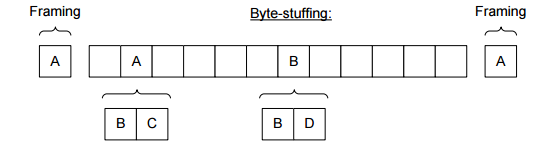
\includegraphics[width=1\linewidth]{Subpages/Billeder/Linklag}
\caption{Linklag protokollen}
\label{fig:Linklag}
\end{figure}

\section{Send funktion}
Til vores send funktion anvender vi v24Putc() som sender en karakter via det fysiske lag, som her er implementeret ved hjælp af en seriel opkobling mellem de to virtuelle maskiner

Vi starter med at sende vores startbit; Karakteren 'A'. 
Dette sikrer at bufferen er tom og array'et på modtager siden er klar til at modtage en ren besked. 
Derefter gennemløbes en if-else-løkke hvor der tjekkes for hvilken karakter der ligger i bufferen som skal indeholder de data der skal sendes; buff[]. Såfremt at karakteren der ligger i buff[] er et A, vil der blive sendt et B efterfulgt af et C. Hvis der ligger et B i buff[] sendes karakterene B efterfulgt af et D. Til slut sender vi stopbittet: igen karakteren A, så modtageren ved, at beskeden er afsluttet.

\section{Receive funktion}
Vores Recieve funktion har den omvendte funktionalitet af send funktionen. Her bruger vi v24Getc() for at hente en byte ad gangen fra det fysiske lag, men da den modtages som en int, typecaster vi den om til en char.\\ Herefter går vi igang med dekodning af vores besked. Da vi forventer at få karakteren A som startbit og stopbit, skal vi vide hvornår vi har modtaget det første A. Dette gøres ved at sætte START$\_$FLAG højt, når startbittet er modtaget. Herefter vil et efterfølgende A indikere at meddelelsen er slut, og vi terminerer linklaget.\\ Modtages karakteren B, testes der med en switch for, om den efterfølgende karakter er enten et C eller et D. Hvis det er et C, returneres karakteren A i bufferen. Hvis det er karakteren D returneres karkateren B i bufferen. Alle andre karakterer bliver direkte overført til bufferen som sendes videre op i transportlaget. Selve receive funktionen returnerer længden af den læste besked.
